
\begin{figure}[t]
\begin{centering}
    {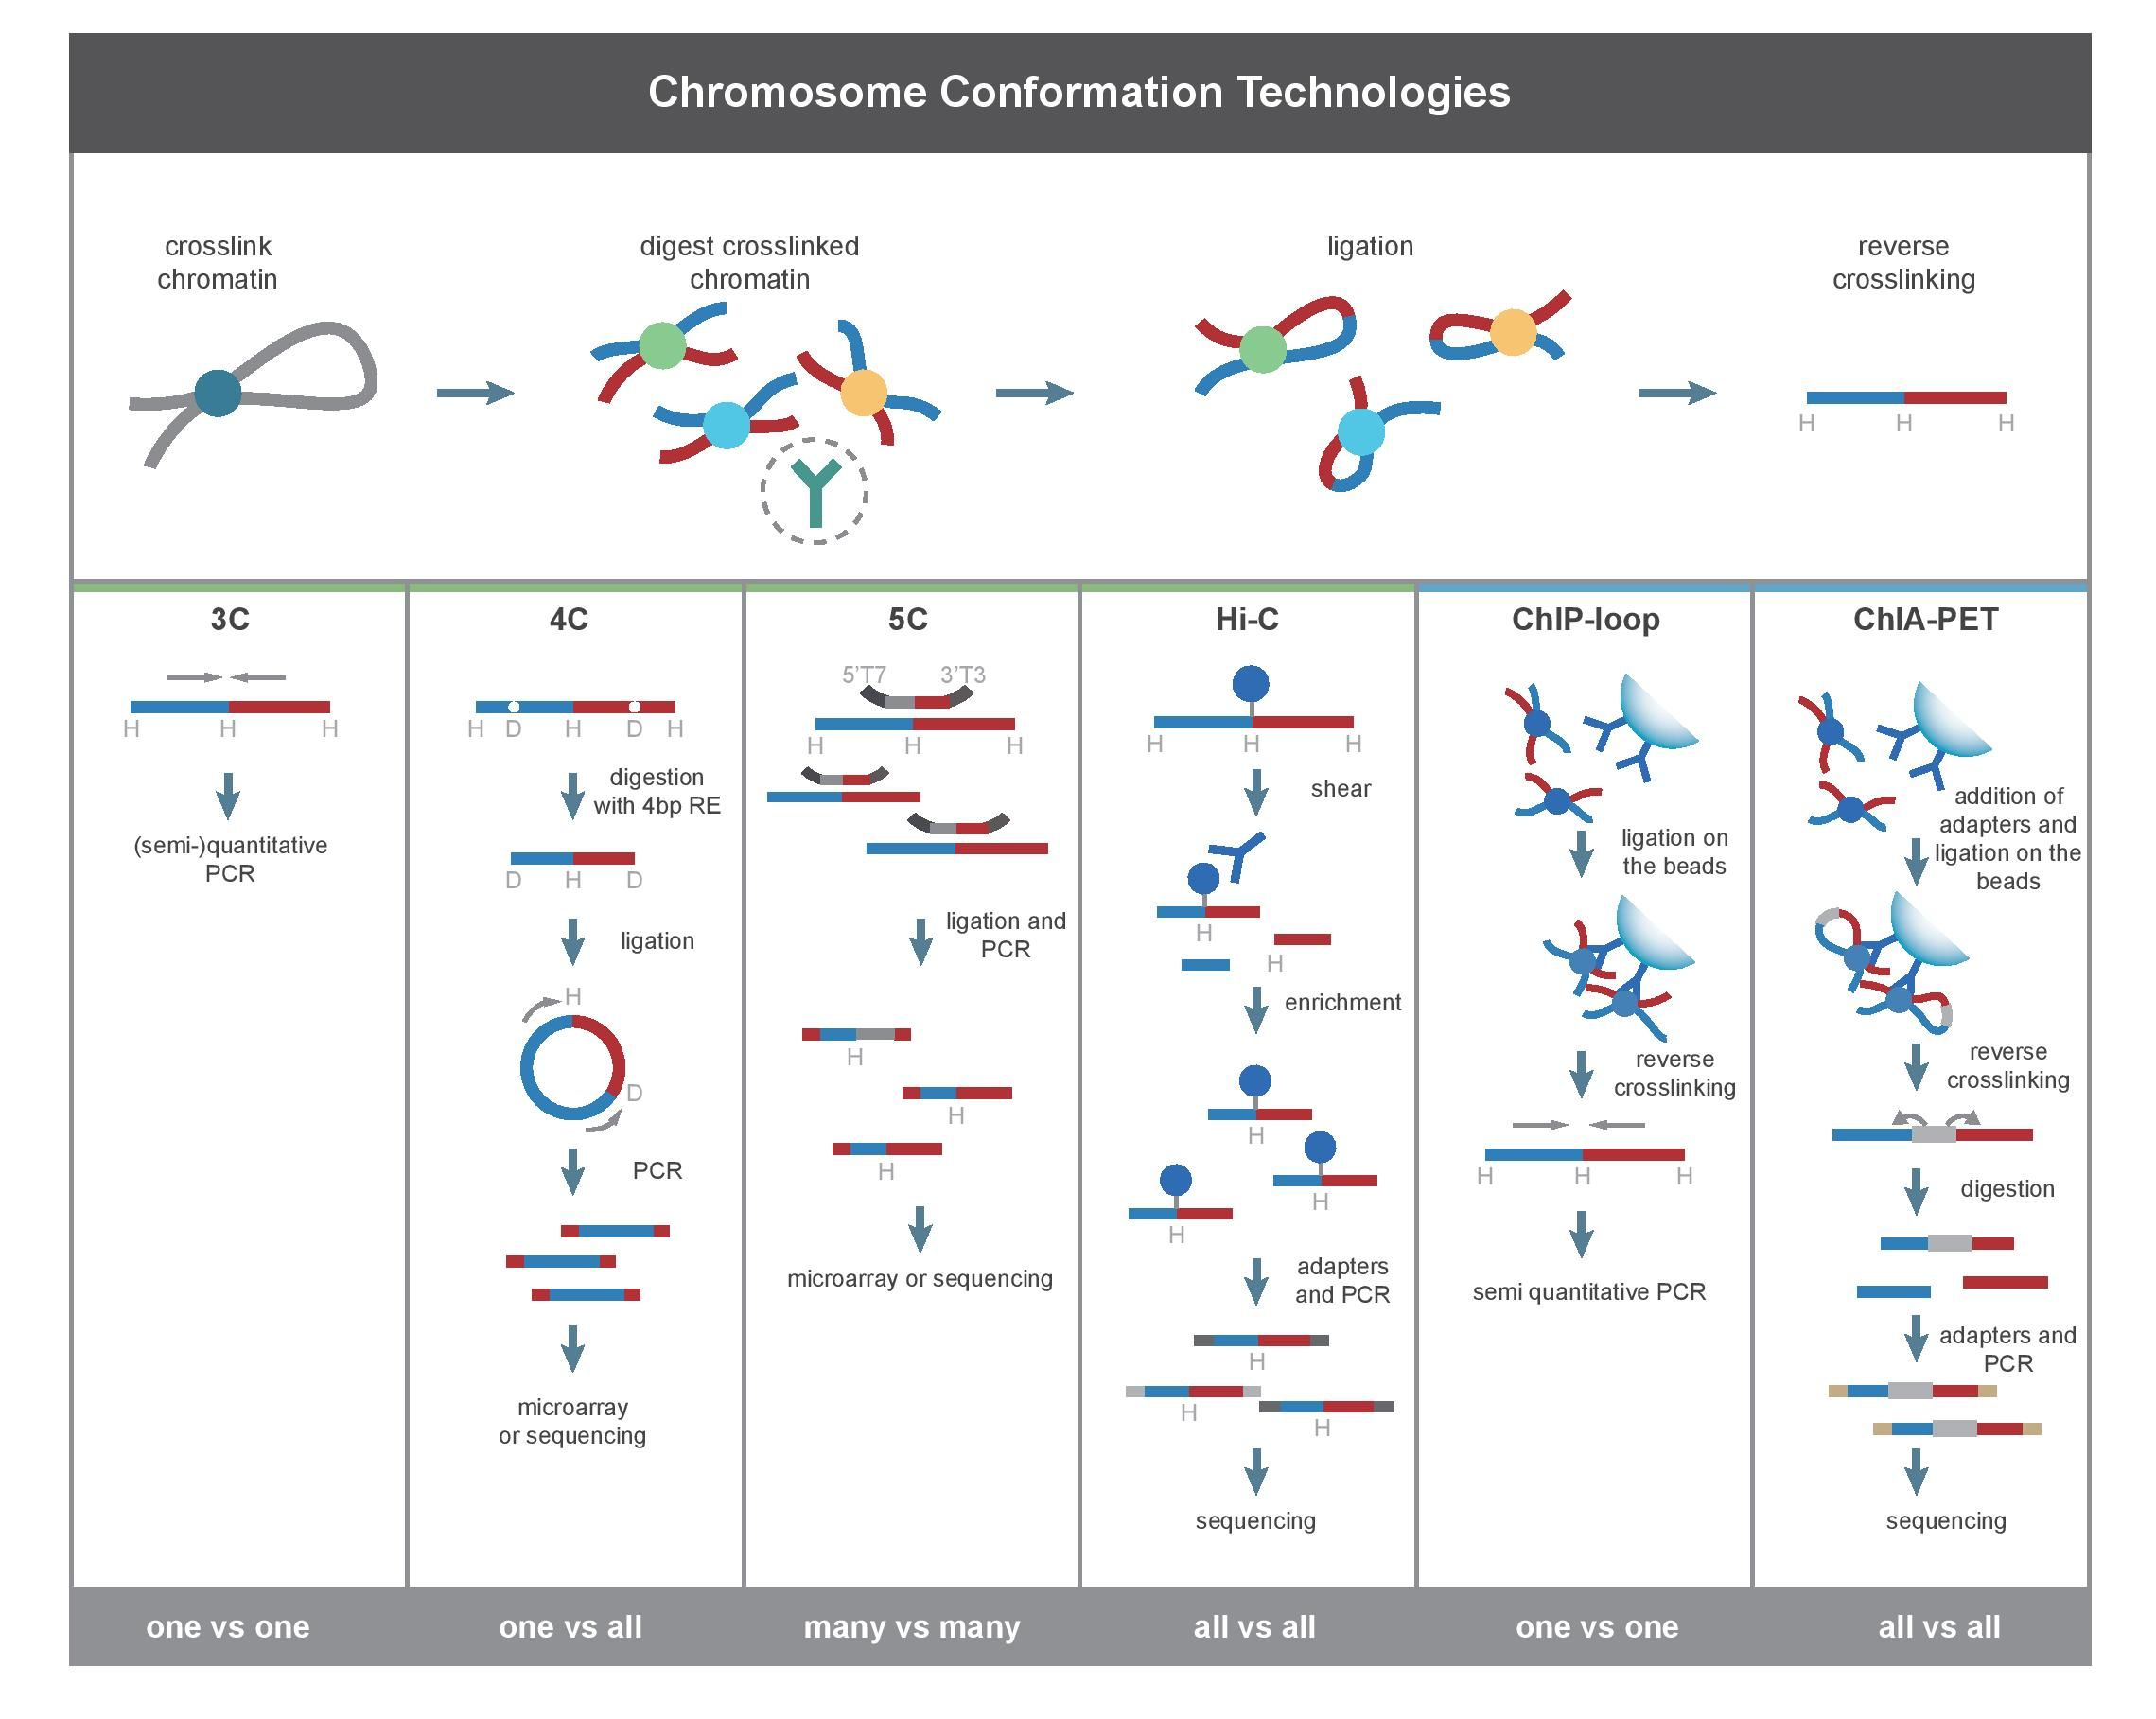
\includegraphics[scale=0.75]{figures/background/Chromosome_conformation_techniques.jpg}}
    \caption[Comparison between 3-C and its derived methods]
    {\textbf{Comparison between 3-C and its derived methods.}
    Clearly seen can be why 3-C, 4-C, 5-C and Hi-C are commonly referred to as
    3-C-based techniques.
    % ChIP-loop and ChIA-PET have these steps in a modified
    % version as well.
    \\ \\ Image from \cite{Li2014}.}
    \label{fig:comparison3C}\label{fig:cct}
\end{centering}
\end{figure}



